\documentclass[11pt, letterpaper]{article}
\input{../../../../report.tex}
%\usepackage{titlepageBU}
\title{Dynamics of the Delayed Logistic Map}
\date{December 2nd, 2024}
\graphicspath{{../figures}}
\usepackage{url}
\DeclareMathOperator{\iin}{int}
\begin{document}
\maketitle
\begin{abstract}
	The dynamics of a delayed formulation of the logistic map are investigated numerically \cite{text}. We use numerical evidence to conjecture that the delayed logistic map behaves chaotically as defined in \cite{devaney}, and describe in depth the end behavior of the seed $(0.1,0.2)$. The biological implications for any system that evolves similarly to \eqref{eq:7} are discussed.

	Unfortunately I made an important mistake while doing my writeup and was unable to complete some of the numerics that I wanted to complete. I have written a short reflection at the end of section \ref{sec:4} that discusses this in more length.
\end{abstract}
\section{Introduction}\label{sec:1}
Ordinary differential equations (ODEs) have applications throughout the sciences, especially in those concerning population modeling. The logistic equation
\begin{equation}\label{eq:1}
	P'(t)=kP\left(1-\frac{P}{N}\right)
\end{equation}
is the most famous example of such a model, in which the population $P(t)$ evolves through time subject to some biological mechanism and limiting factor described by the $1-\frac{P}{N}$ term. However, its simplicity is due to the many approximations the model makes, and it's not obvious that the model should be applicable in highly nuanced circumstances involving many independent variables. One of these assumptions is that biological mechanisms happen fast enough that any lag is negligable \cite{hutchinson}, but in reality this is often not the case. Delay differential equations (DDEs) are a class of differential equations related to both a solution $y(t)$, and the solution at some previous point in time $y(t-\tau )$, $0<\tau $. A DDE reformulation of the logistic proposed in \cite{hutchinson} now known as the delayed logistic model, or Hutchinson's equation, takes the form
\begin{equation}\label{eq:2}
	\frac{\mathrm{d}P}{\mathrm{d}t}=kP(t)\left( 1-\frac{P(t-\tau )}{N} \right)  
,\end{equation}
where $\tau \in\mathbb{R}^+$ is some fixed lag parameter. Unlike \eqref{eq:1}, which has well known solutions, \eqref{eq:2} currently has no known closed form solutions, and much of the successful analysis on the dynamics of the system has been qualitative \cite{ddes}.

Another modified representation of \eqref{eq:1} as given in \cite{text} is as a discrete system, where the population at time $n$ is modeled by a sequence $\left\{ y_{n} \right\}_{n=0}^\infty $ where
\begin{equation}\label{eq:3}
	y_{n+1}=ky_n\left( 1-\frac{y_n}{N} \right)
.\end{equation}
Equation \eqref{eq:3} is known as the logistic map, or the discrete logistic equation, and is a classic example of how chaotic behavior can arise from relatively simple systems. Using the same logic as Hutchinson in \cite{hutchinson}, we can modify the logistic map to account for some time delay in biological processes by also considering the previous iterate:
\begin{equation}\label{eq:4}
	y_{n+1}=ky_n\left( 1-\frac{y_{n-1}}{N} \right) 
.\end{equation}
Equation \eqref{eq:4} is known as the delayed logistic map, and is the simplest formulation of a delayed variant of the logistic map. We can simplify the equation slightly by considering $y_n$ to represent the ratio of the current population to the carrying capacity of the system, and redefine the equation as
\begin{equation}\label{eq:5}
	y_{n+1}=ky_n\left( 1-y_{n-1} \right) 
.\end{equation}

To further investigate \eqref{eq:5}, we can define a new sequence $\left\{ x_{n} \right\}_{n=0}^\infty $ where $x_0\in\mathbb{R}$ is fixed and $x_{n}=y_{n-1}$ for all $n\geq 1$. We can then define $F_k : \mathbb{R}^2 \to \mathbb{R}^2$ as the mapping
\begin{equation}\label{eq:6}
	F_k(x,y)=\left( y,ky\left( 1-x \right)  \right) 
,\end{equation}
and we have
\begin{equation}\label{eq:7}
	\left( x_n,y_n \right) =F_k(x_{n-1},y_{n-1})
.\end{equation}

We will numerically iterate \eqref{eq:7} to explore long-term behavior of the function $F_k$ for parameter values $k\in[1.5,2.5]$, and from this analysis deduce behavior of $\left\{ y_n \right\}_{n=0}^\infty$. We will explore bifurcation values for $k$, and classify the behavior of the system before and after bifurcations occur.

\section{Bifurcation Analysis}\label{sec:2}
Before we can preciely analyze the long-term behavior of the orbits of $F$, we need to identify bifurcation points and classify system behavior between these points. For our initial analysis, we took $(x_0,y_0)=(0.1,0.2)$ to be the seed for \eqref{eq:7}, and calculated 200 iterations of $F_k$ for $k$ values along the interval $[1.5,2.5]$ separated by $0.01$. In addition to some very beautiful graphs, we were able to identify that at least one bifurcation point exists, and likely at least two.

We found that there exists some $k_b$ such that $y_n \to -\infty$ as $n\to \infty$. Using the fact that any $y_n<0$ always diverged to $-\infty$\footnote{Shown later.}, we used a binary search algorithm (code \hyperref[code:1]{1} ) to find a precise value of $k$ for which $y_n$ would go negative. We found the value of $k_b$ to be about $2.271$ at 100 billion iterations of $y_n$ and a precision in $ k$ of less than $10^{-15}$. We will call this the infinity bifurcation, and denote it $k_{\infty}$.

For all $k<k_\infty$, the sequence appeared bounded by $0<y_n<1$ for all $n$, and there appeared to be a possible second bifurcation. As seen in figure \ref{fig:1}, for smaller $k$ values, $y_n$ appeared to approach a fixed solution, whereas for larger $k$ values, the system appears to cycle about a set of periodic points, and a boundary region inside which the function did not exist appeareed to exist.

\begin{figure}[ht]
	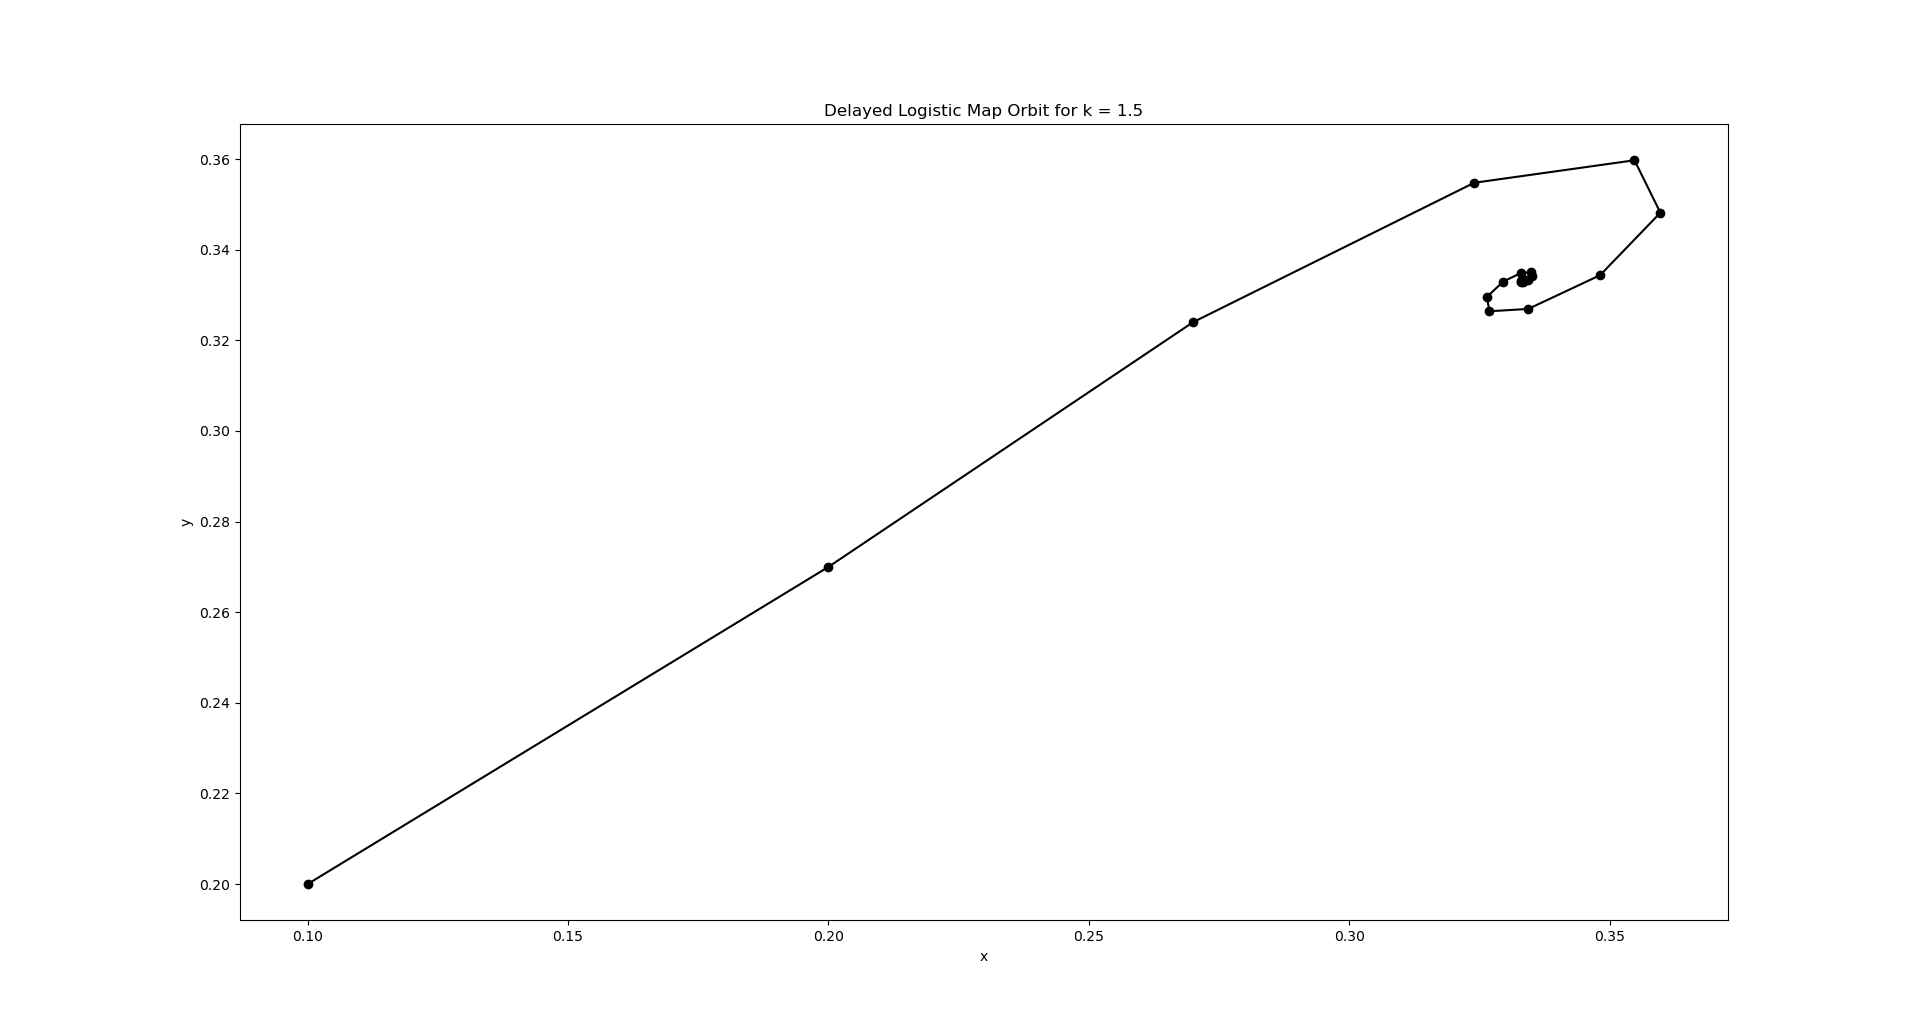
\includegraphics[scale=0.16]{k15.png}
	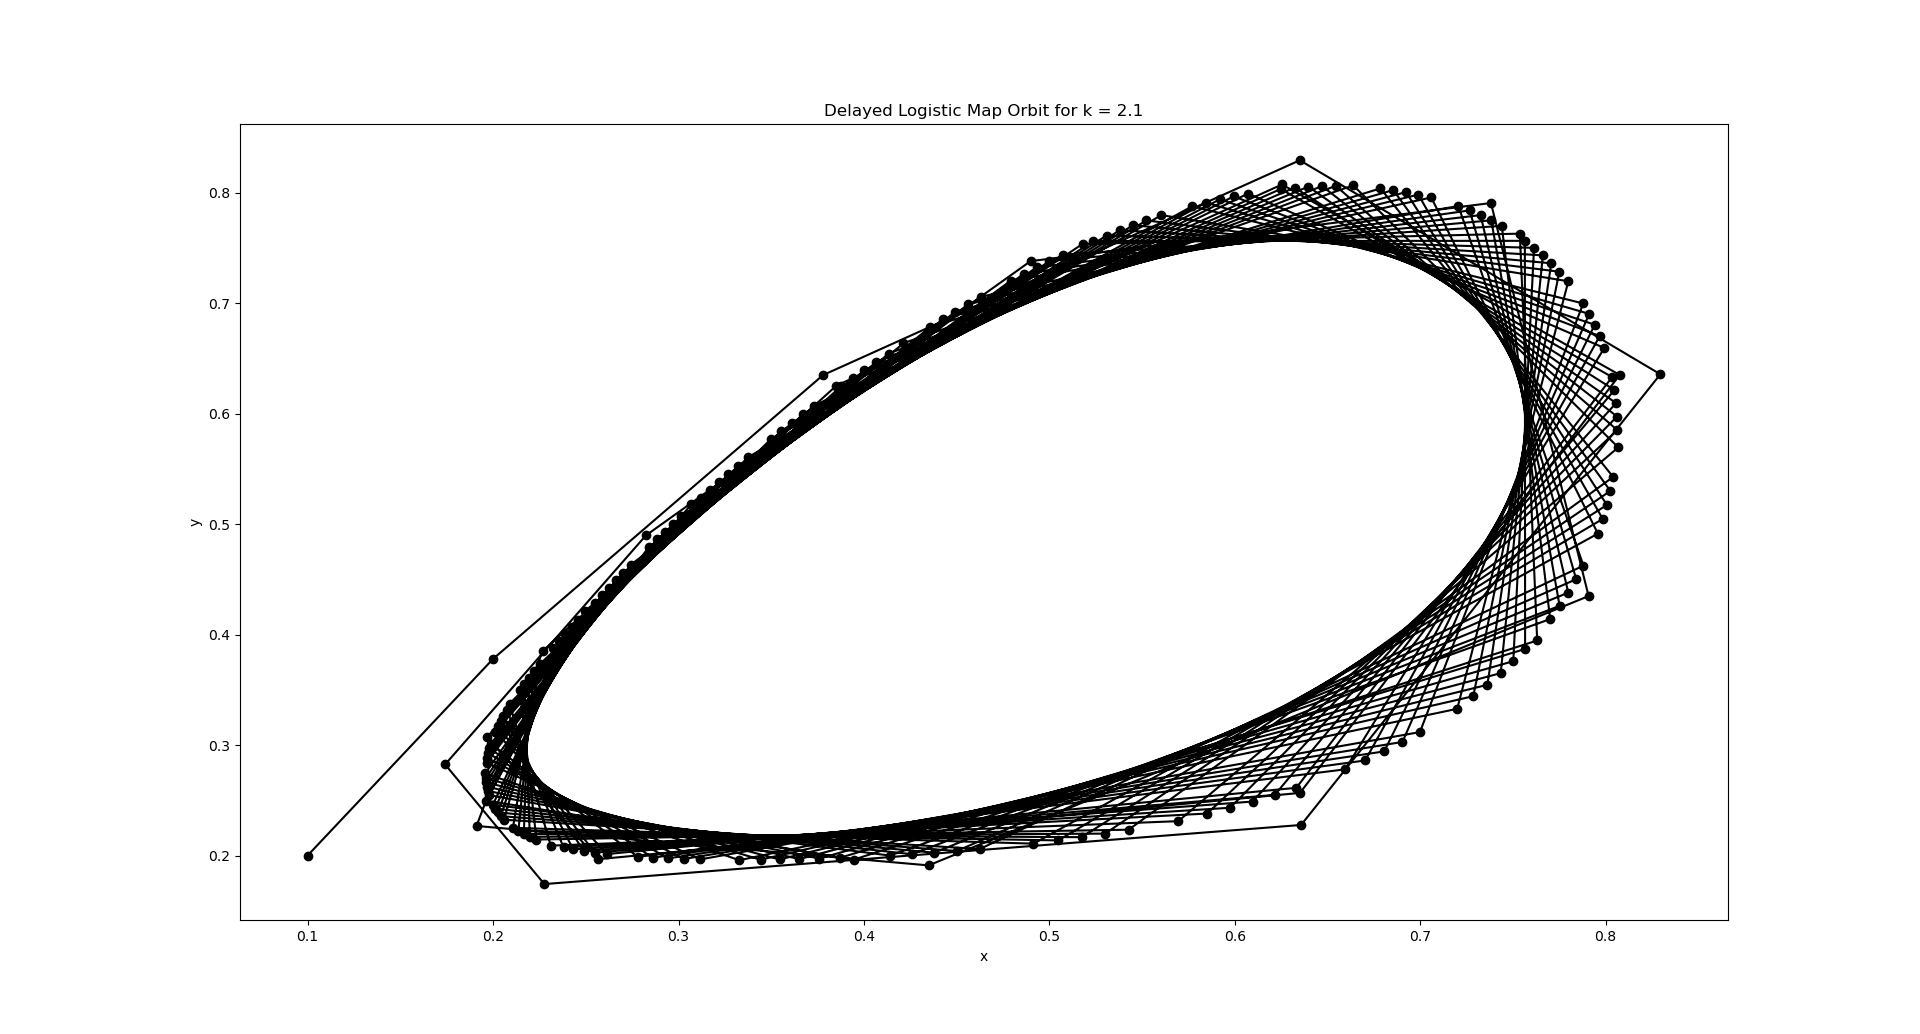
\includegraphics[scale=0.16]{k21.png}
	\centering
	\caption{Orbits in Phase Space for Select $k$-values}\label{fig:1}
\end{figure}

Although it is possible that longer iterations could cause these pictures to have similar behavior, this seems unlikely and it appears as if another bifurcation has occured. To investigate, we used code \hyperref[code:2]{2} to plot the bifurcation diagram for \eqref{eq:7} for $k$-values along $[1.5,k_{\infty})$. We iterated $y_n$ 100000 times, incremented $k$ by $0.00002$ along the interval $[1.5,2.27]$, and plotted the last 200 data points for each iteration of $k$. We observed behavior equivalent to that seen in figure \ref{fig:2}, although figure \ref{fig:2} has less data points plotted, simply for neatness.

\begin{figure}[ht]
	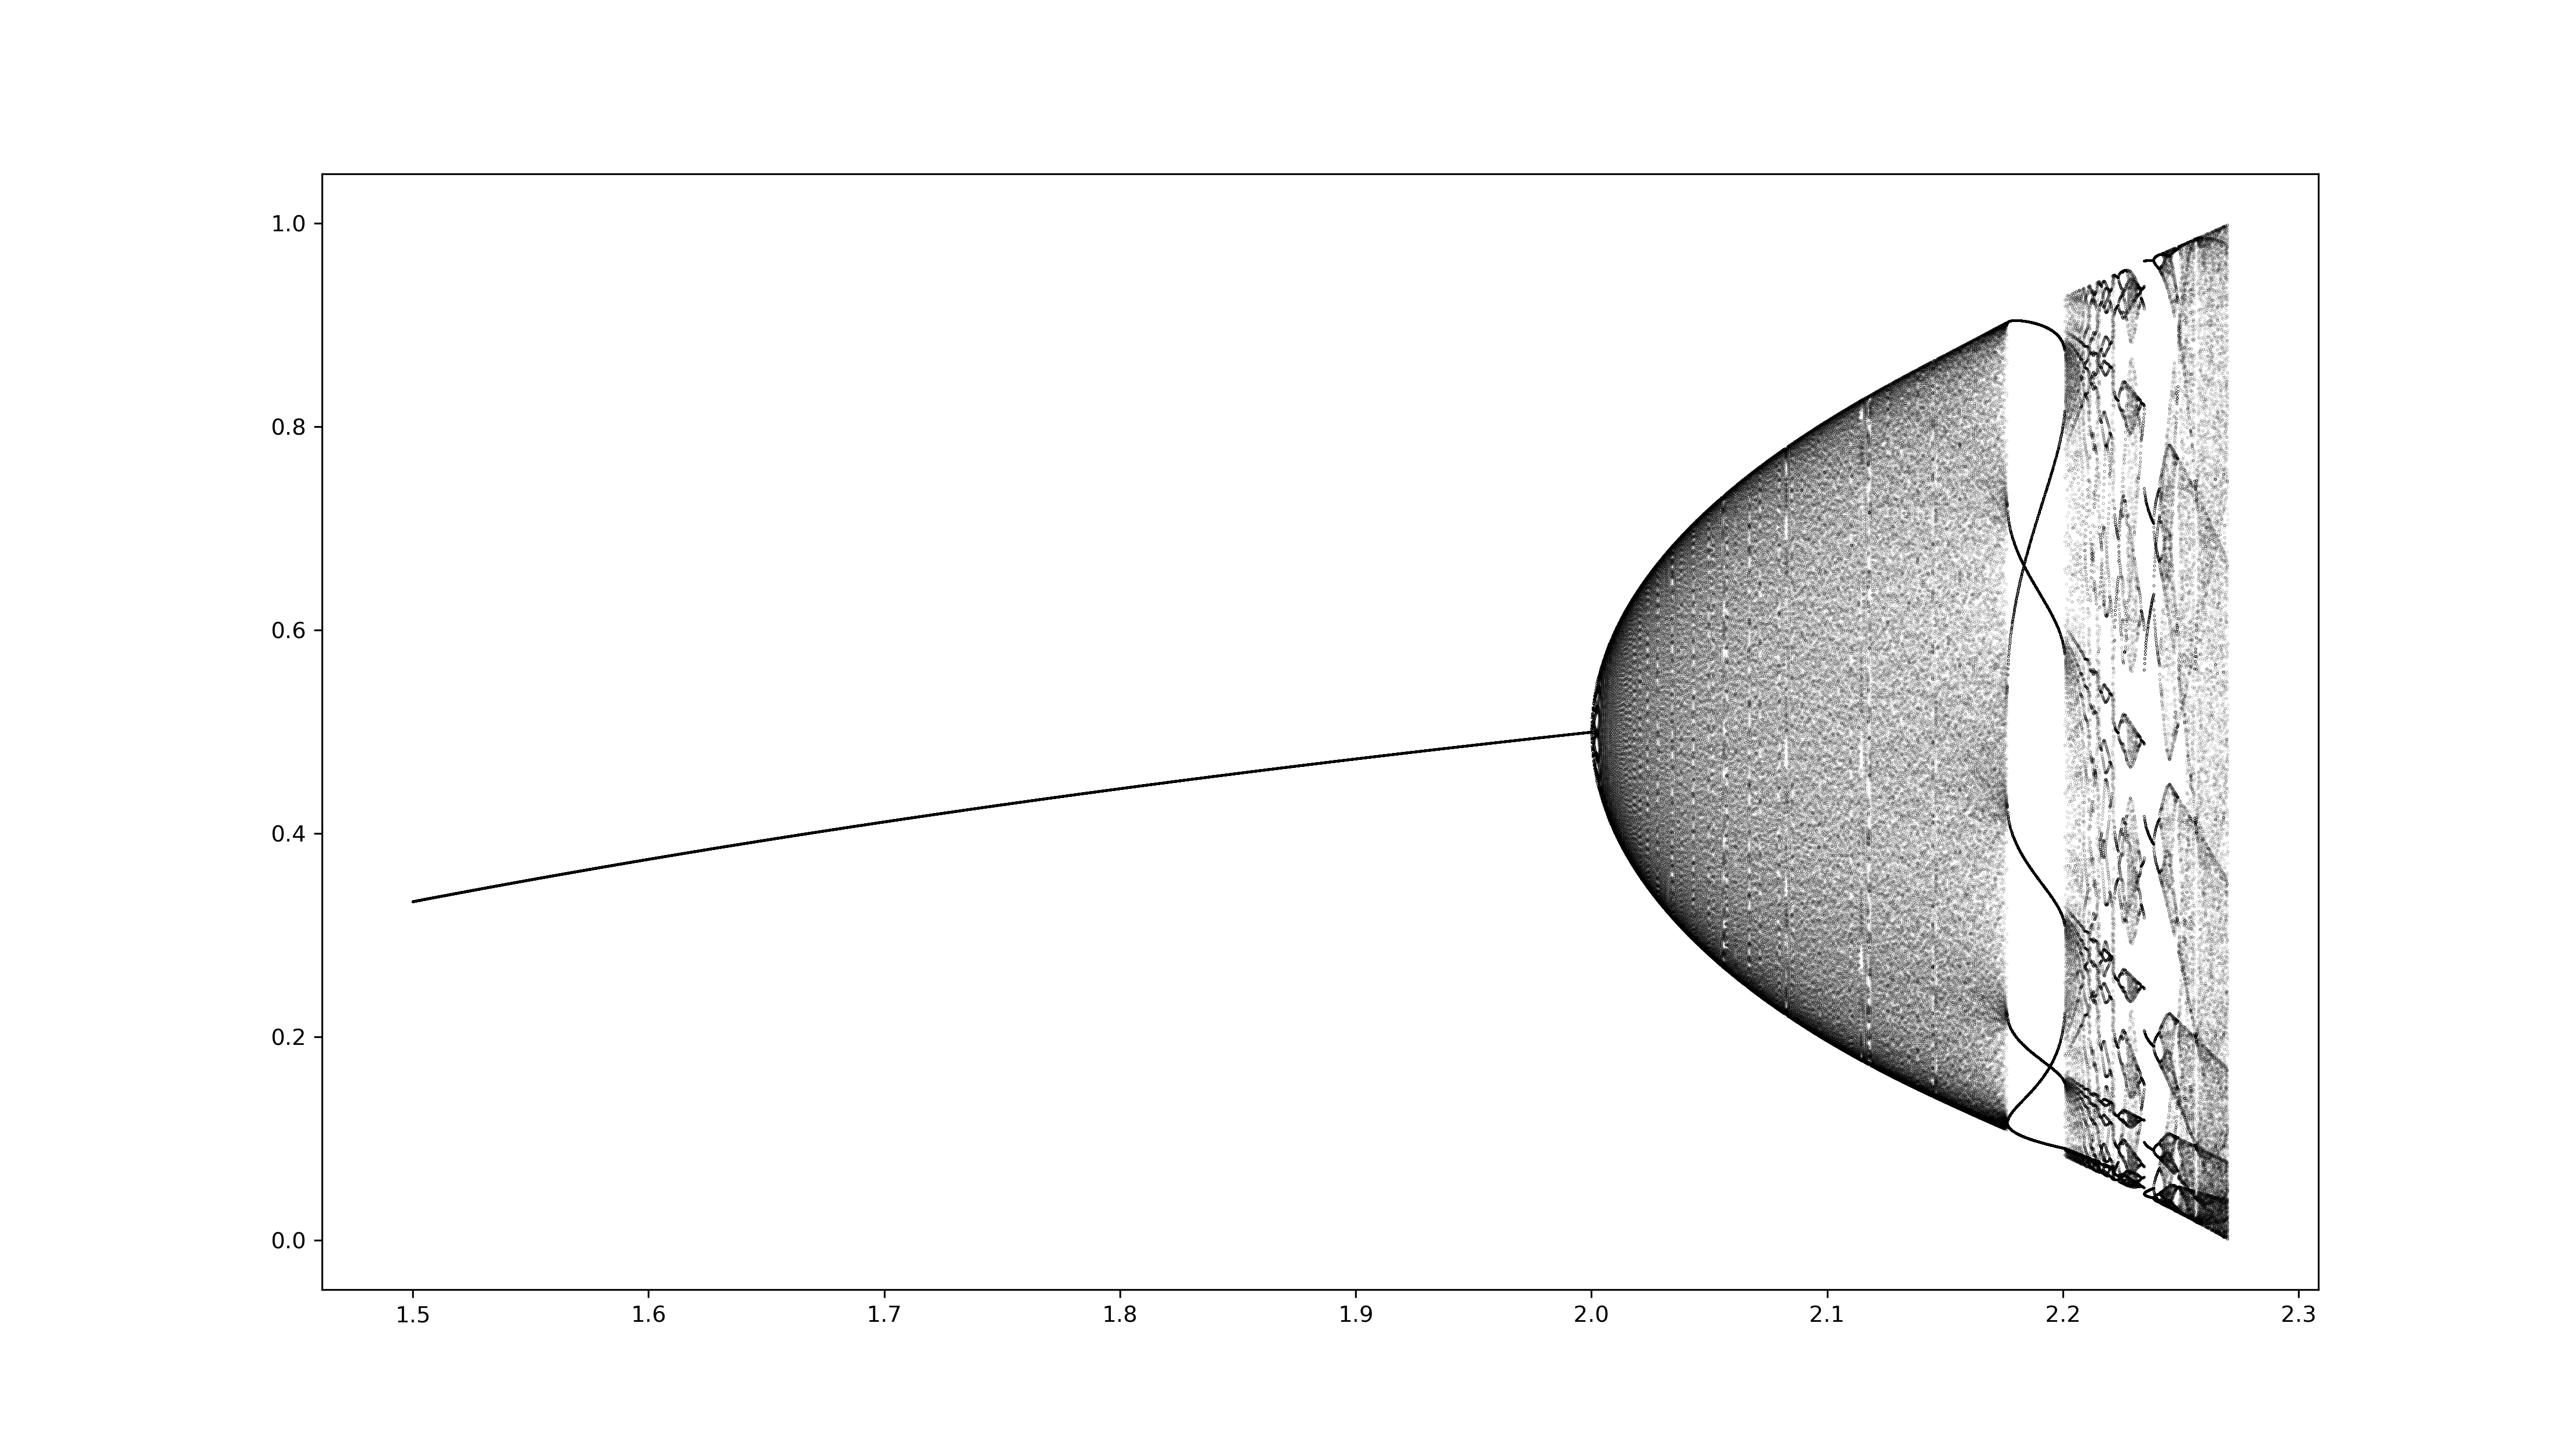
\includegraphics[scale=0.4]{correct.png}
	\centering
	\caption{Bifurcation Diagram for \eqref{eq:7}}\label{fig:2}
\end{figure}

Using figure \ref{fig:2}, we can extract quite a lot of informtation about the bifurcations of the system, which will allow us to later identify the end behavior of the system \eqref{eq:7}. First, we note that for $k\in[1.5,2)$, the system approaches a single value, which will be shown later to be $\frac{k-1}{k}$. For $k\in (2,k_{\infty})$, the system appears to experience chaotic behavior.  There is an island of stability ranging from around $k=2.17$ to $2.2$, where the orbits are either completely periodic, or cluster extremely heavily about a maximum of $7$ points. Multiple bifurcations occur within this region, as the number of points spontaneously increases and decreases by 1, visualized by the intersecting lines within this region. After this region, the system decends back into chaos, but with various voids in which no endpoints of the iteration occur for some reason.

Since the logistic map attractor around the onset of chaos is well known to be a fractal with Hausdorff dimension around 0.538 \cite{grassberger}, and figure \ref{fig:2} bears significant resemblence to the bifurcation diagram for \eqref{eq:3}, it's reasonable to assume the attractor for \eqref{eq:7} may also have fractional dimension. However, since \eqref{eq:7} requires two initial conditions and thus behaves at least two-dimensionally, its attractor $A$ will be some subset of $\mathbb{R}^2$, rather than $\mathbb{R}$.
\section{Analysis of End Behavior}\label{sec:3}
\subsection{Region of Stability}
A fixed point $(x_n,y_n)$ is any point such that $F(x_n,y_n)=(x_n,y_n)$. By \eqref{eq:6}, this implies $x_n=y_n$ for some $n$, and by induction it can be shown this holds for all $n'\geq n$. Therefore, we require $x_n=y_n$ for any fixed point, and by \eqref{eq:6} we can characterize fixed points as any $y_n$ satisfying
\begin{equation}\label{eq:8}
	y_n=ky_n\left( 1-y_n \right) 
.\end{equation}
This is precisely the same as a fixed point of the logistic map \eqref{eq:3}. By the quadratic formula,
\begin{equation}\label{eq:9}
	ky_n^2+(1-k)y_n=0
.\end{equation}
We find that $\left\{ 0,\frac{k-1}{k} \right\} $ are the fixed points of the system. This explains behavior seen in section \ref{sec:2}; we observed that for $1.5\leq k<2$, the solutions appeared to approach some fixed point, which we can now describe as an attractive fixed point. For $k>2$, the qualitative nature of the fixed point has changed in a bifurcation. Magnifying the region of figure \ref{fig:2} near $k=2$ shows that this bifurcation appears similar to a period doubling bifurcation, but the period appears to double so rapidly that we cannot view individual period doublings with the computational power at our disposal.

\subsection{Region of Chaos}
Consider the following formal definition of chaotic behavior, as formulated by Devaney in \cite{devaney}.
\begin{definition}[Chaos, \cite{devaney}]\label{dfn:1}
	Let $X$ be a topological space, and let $f : X \to X$ be a function. We say $f$ is chaotic if
	\begin{itemize}
		\item There exists $\delta >0$ such that for any $x\in X$ and any neighborhood $N$ of $x$, there exists $y\in N$ and $n>0$ such that $\left| f^n(x)-f^n(y) \right| >\delta $. This property is called sensitivity to initial conditions.
		\item For any open sets $U,V\subset X$, there exists $n>0$ such that $f^n(U)\cap V\neq \varnothing$. This property is called topologically transitive.
		\item Periodic points of $f$ are dense in $X$.
	\end{itemize}
\end{definition}
This author was unable to find any formal proof that the delayed logistic map satisfies definition \ref{dfn:1} for some choice of $k$, so the problem will be tackled numerically for a choice of $k=2.1$ within the region of chaos. We choose $k=2.1$ based on the apparent homogeneity of the distribution of $y_n$ values along the attractor in figure \ref{fig:2}, and also due to the fact that the attractor  appears to be some sort of smooth curve or Jordan curve. Not having to deal with the voids observed after the period of stability simplifies the analysis, but further analysis should explore these regions further.

\begin{theorem}\label{thm:1}
	For any choice of $k\in (2,k_\infty)$ and for any $n\in\mathbb{N}$, $y_n\in (0,1)$.
\end{theorem}

Theorem \ref{thm:1} states that the solution remains bounded by $0$ and $1$ for all $n$. It should be obvious that this statement is equivalent to being bounded by 1 from above, as $y_n>1$ implies that $y_{2n}=y_{n+1}(1-y_n)<0$ due to the $1-y_n$ term, and thus the system would not be bounded below from 0. Theorem 1 is left unproven because this author had absolutely no idea how to complete a proof without formulating an extremely messy and possibly nonexistant general formula for $y_n$ given initial conditions $(x_0,y_0)$ and performing analysis I did not have time to complete. It can be seen, however, from figure \ref{fig:2} that the solutions do in fact remain bounded for very large $n$, and it is not unreasonable to suppose this theorem holds.

There are various formal definitions of attractors in the literature, but in general, an attractor $A$ is a region with an open neighborhood $N_A$ such that for all $x\in N$, as $n\to \infty$, $f^n(x)\to y$ for some $y\in A$. More intuitively, an attractor is a region that all points nearby evolve to as the dynamical system evolves. This definition immediately implies $f(A)\subseteq A$.

Based on figure \ref{fig:3}, the attractor appears to be some smooth Jordan curve $A$ in $\mathbb{R}^2$. This would explain why each point $(x_n,y_n)$ appeared to lie on this single curve, as there would then exist some homeomorphism $\gamma : \mathbb{R}^2 \to \mathbb{R}^2$ such that $\gamma(\mathbb{S}^1)=A$, where $\mathbb{S}^1$ is the unit circle. The map $F_k$ could then be seen as a linear map $T\in \operatorname{SO}(2) $ on $\mathbb{S}^1$ such that $F_k(x_n,y_n)=\gamma \left( T\left( \gamma ^{-1}(x_n,y_n) \right)  \right) $. Although we are unable to identify such a homeomorphism $\gamma $, this is an interesting aside that may warrant further research. One idea would be to approximate a parameterization of $A$ using some code, and find a homeomorphism from $\mathbb{S}^1$ to some perturbation of this parameterization.

\begin{figure}[ht]
	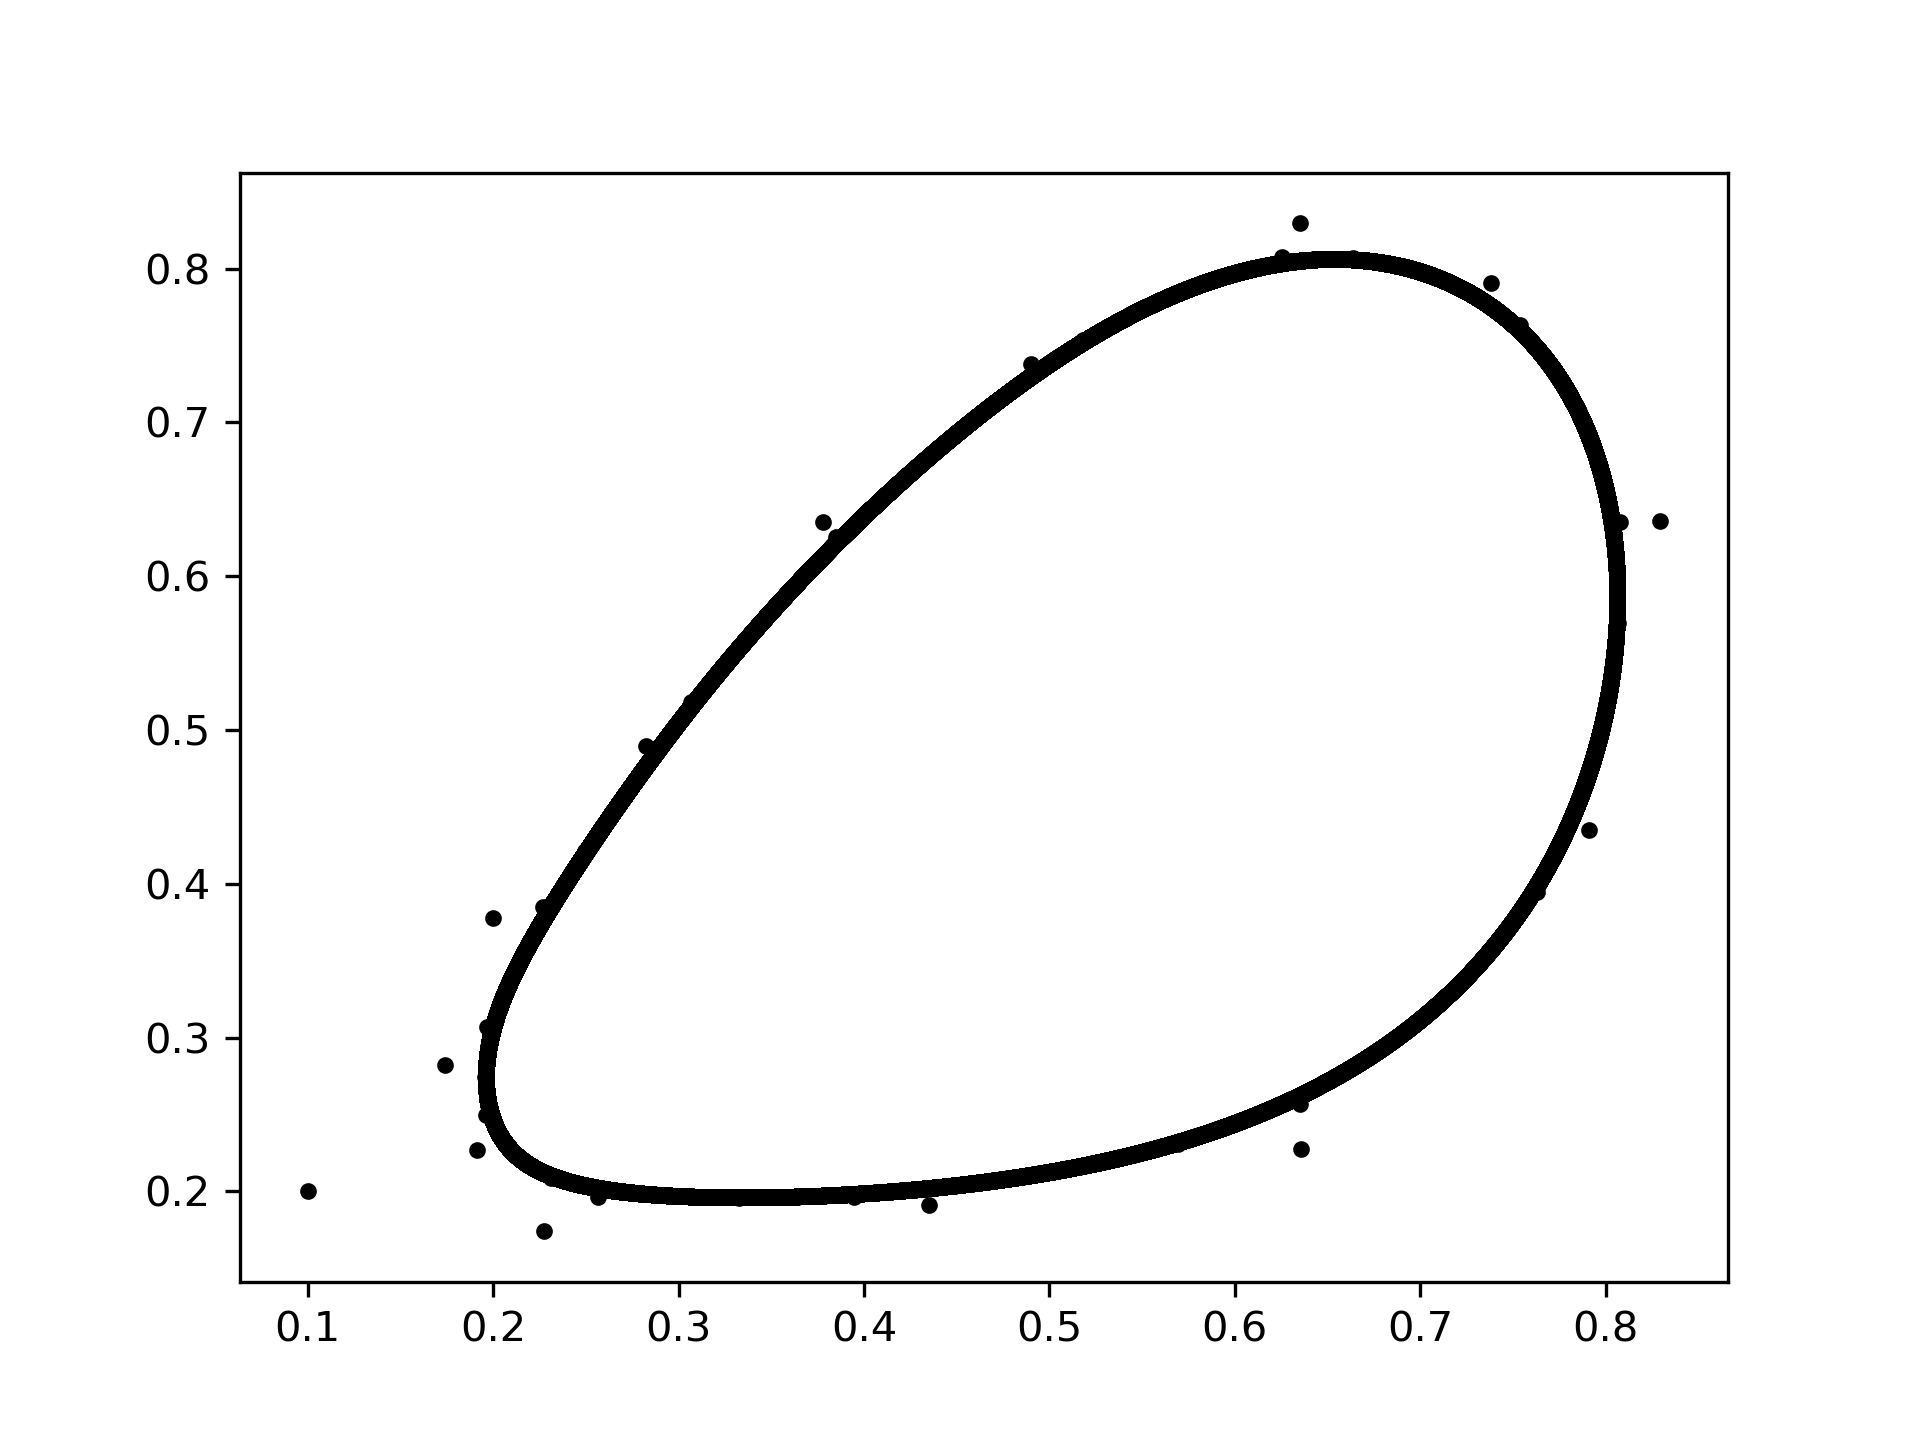
\includegraphics[scale=1]{Attractor.png}
	\centering
	\caption{First 100000 Iterates of $y_n$}\label{fig:3}
	\centering
\end{figure}

Nonetheless, $A$ appears to take the form of a smooth, simple closed curve, and we want to show $F_k : A \to A$ is a chaotic system for our choice of $k$. To do this, we will first need a numerical method of approximating the curve $A$. To do this, we will compute a large number $p$ of points $(x_n,y_n)$ for some initial seed, and delete the first 100 iterations of $F_k$ to eliminate all points far from the attractor. We will then define  $\mathcal{A} (p)$ to be the polygon formed by connecting each point to the two nearest points using a straight line. This is a suitable approximation for $A$, and as  $p\to \infty$, we should have $\mathcal{A} (p)\to A$.

This approximation is also nice because we want to use the subspace topology on $A$, meaning distance will be defined via the usual metric on $\mathbb{R}^2$. Since $A$ is a one-dimensional structure, the intersection of any open ball $B_r(x)$ with $A$ will be a one-dimensional line with endpoints $a,b$ having $d_{\mathbb{R}^2}(a,b)\leq r$. Moreover, the interesctions of the basis for the metric topology on $\mathbb{R}^2$ will form a basis for the subspace topology on $A$, so we can consider the topology to be generated by the set of intersections of $A$ with open balls of a point on $A$. That is, if $\mathcal{B} $ is defined as
\begin{equation}\label{eq:10}
	\mathcal{B} =\left\{ A\cap B_r(x) \mid x\in A\land r\geq 0 \right\} 
,\end{equation}
then $\mathcal{B} $ is a basis for the subspace topology on $A$.

By definition \ref{dfn:1}, we wish to show that every open set of $A$ contains at least one point $(x_n,y_n)$. We can approximate this on $\mathcal{A} (p)$ by showing that if there are $p-100$ points on $\mathcal{A} (p)$, then there should be no points further apart than $ 2\ell (A) / (p-100) $ for $\ell (A)$ the arclength of $A$. If such points exist, then there are neighborhoods on $\mathcal{A}(p)$, and thus approximate neighborhoods of $A$, of radius greater than or equal to $\ell (A) / (p-100)$ that do not contain an element of $\mathcal{A} (p)$. There may be points this approximation does not account for that are this distance, or further, from any points along $\mathcal{A}(p)$. However, since the attractor appears to locally resemble $\mathbb{R}$, the approximation should work fairly well on low scales. We can quantify the amount of neighborhoods that do not contain such a point using a measure function, and we wish to show the periodic points of $F_k$ are dense almost everywhere with respect to the measure, or that they tend to 0. This measure would simply be the arclength of the segment for which no neighborhoods of this radius contain a point.

Due to needing to turn this assignment in soon, I will not rigorously define this measure, but I will note that due to the finite nature of $p$, the measure will simply be the length of a finite number of intervals along $A$, and thus the definition can be similar to that of the Lebesgue measure in order to generate the proper $\sigma $-algebra. We will call this measure $\mu_{\ell } $, and will numerically approximate $\mu_\ell (A)$ by approximating $\ell (A)$, finding all points $(x_n,y_n)$ which are further from all other points by at lesat $2\ell (A) /(p-100)$, and adding up the total distance minus this length. This was a very poor explanation.

We used code \hyperref[code:3a]{3a} to find that the approximate arclength at $p=10^5$ to be $\ell (A)\approx 1.9118341342949094$. We are unfortunately limited by computing power to this value, but we will use this value throughout the remainder of the paper. We then used code \hyperref[code:3b]{3b} to approximate $\mu_\ell (A)$ by the method stated previously. To normalize our results against the arglength of $A$, we also divide by $\ell (A)$ after computing. For $p=10^5$ we find that $\mu_\ell (\mathcal{A} (p))\approx 0.0234$. We computed $\mu_\ell (\mathcal{A} (p))$ for all iterations of $p$ from $10000$ to $100000$, separated by $10000$. Our results are plotted in figure \ref{fig:4}.
\begin{figure}[ht]
	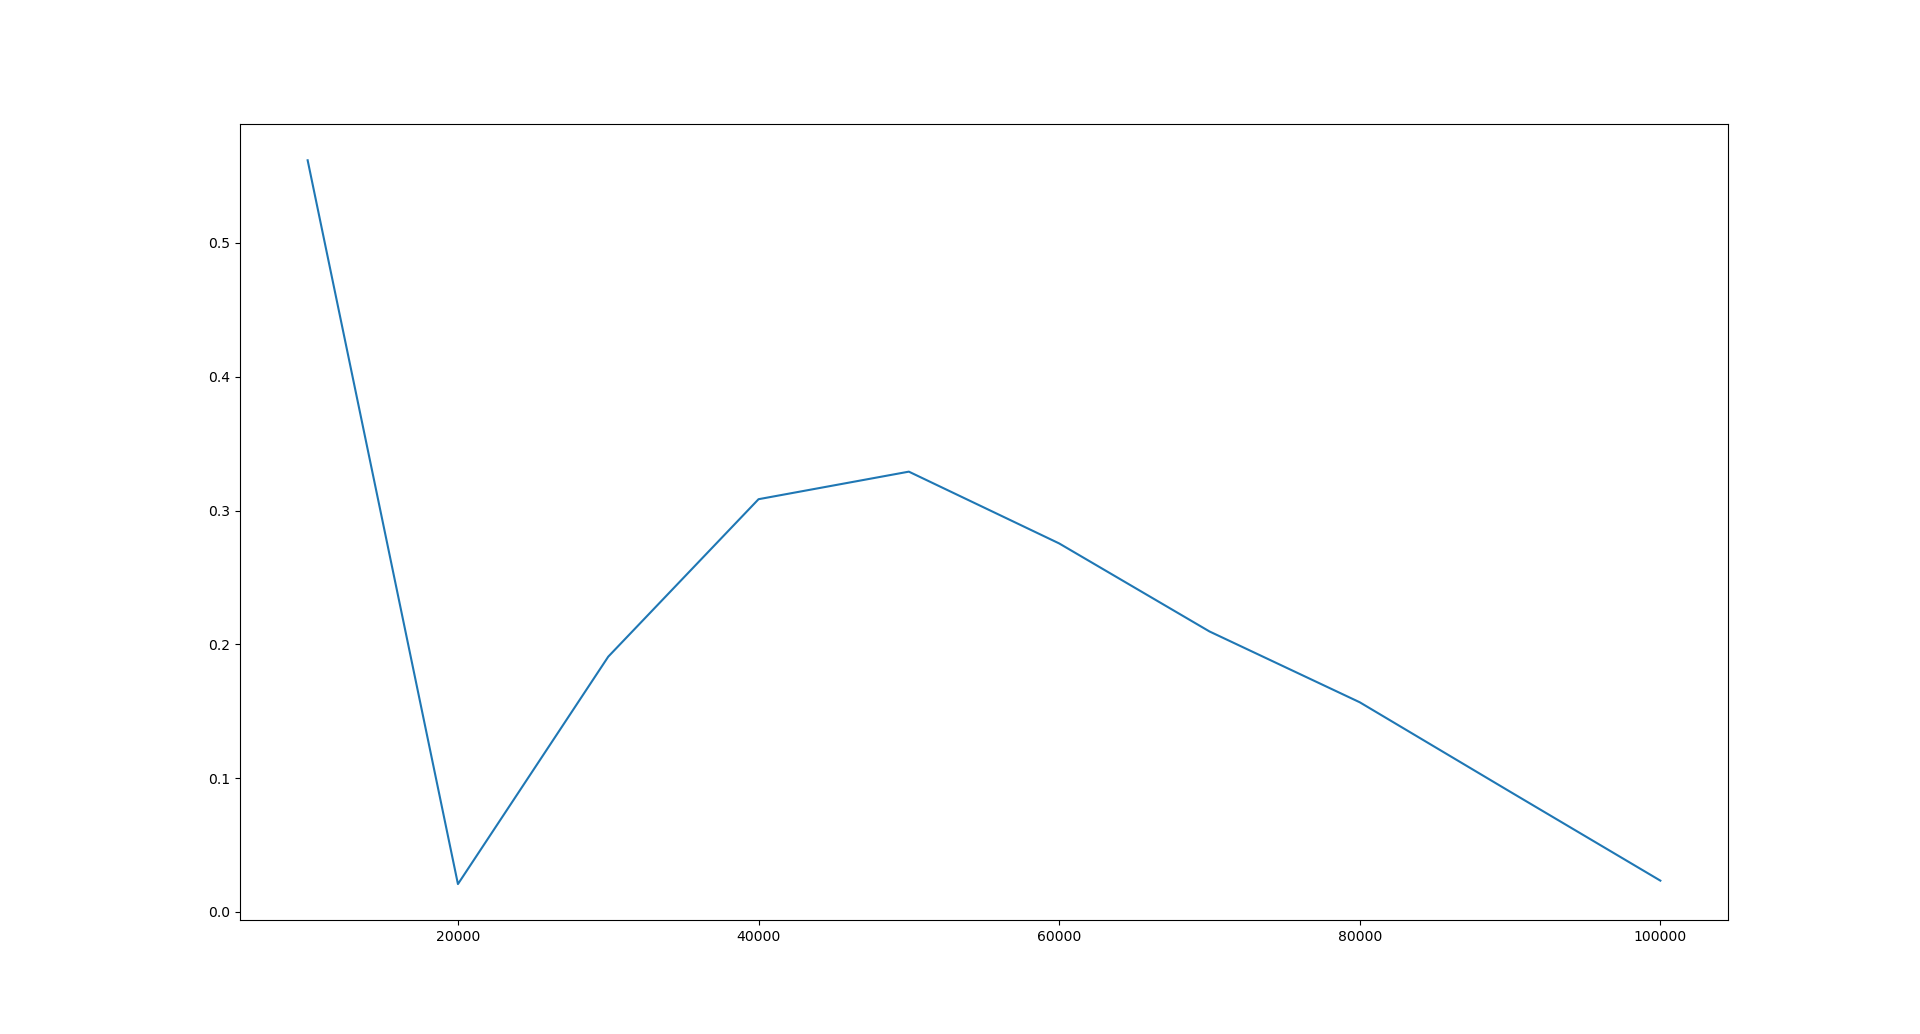
\includegraphics[scale=0.35]{L-measure.png}
	\centering
	\caption{$\mu_\ell $ for varying $p$ values}\label{fig:4}
\end{figure}

Our results are handicapped by our computing power. Although it appears as if $\mu_\ell (\mathcal{A} (p))$ is going to $0$, there is a spike between $p=20000$ and $p=50000$ that implies there may be more behavior beyond the scope of our computability. We will leave this for others to research, but for now we will say that there is some evidence $\mu_\ell $ may tend to $0$, and so the periodic points of this specific orbit may well be dense in $A$.

Unfortunately, this assignment is due soon, and I would feel bad asking for an extension, even though this stuff is really cool. So I do not have time to complete my numerical analysis. I will instead outline how to numerically check the first and second properties of definition \ref{dfn:1}. Using the set of points, you can ask ChatGPT for some code that will construct an approximate parameterization $r(t)$ of the curve using the points such that $r[0,1]\approx A$. Choose some accuracy $p$ and divide $[0,1]$ into $p$ iterates $t_p$ a distance $1 / p$ away from each other. Find $r(t_p)$ for each $t_p$. We will use this to approximate an open cover of $A$ in various neighborhoods of points. However, since equivalent differences in $t$ may induce different arclength differences of $A$, we will find the maximum distance between any two $r(t_p)$ values, and take this to be the width of our neighborhoods.

To check the first propery, for each $t_p$ choose a $t_q$ value extremely close to $t_p$ such that it will be in the maximum number of neighborhoods of $x$, and choose some large $n$. Iterate $F^n(r(t_p))$ and $F^n(r(t_q))$ for all $t_p$ and $t_q$, and show that all $t_p$ attain a distance away from the corresponding $t_q$ of some positive value. Define this value as $\delta $, and property 1 is thus verified down to neighborhoods of the given radius.

To check the second property, you must iterate each  $r(t_p)$ until the set of all points $F^n(r(t_p))$ less than the given radius away from every base point $r(t_p)$. Plot $n$and $p$ along the same axis, and show that it is reasonable that as $p\to \infty$, we will have $n$ remain finite. This will imply that a point in a given neighborhood $U$ will end up in all open balls $V$, and thus $F^n(U)\cap V\neq \varnothing$ for some $n$. This verifies the second property up to $p$, and gives reason to suspect it will hold in general.
\subsection{The Infinity Bifurcation}
The analysis for this section is fairly simple. It can be verified numerically that for $k\geq k_{\infty}$, there will be some $y_n>1$. If $y_n>1$, then $x_{n+1}>1$, and thus
\[
	y_{n+2}=y_{n+1}\left( 1-x_{n+1} \right) <0
.\]
We then have
\[
	y_{n+3}=y_{n+2}\left( 1-x_{n+2} \right) <0
,\]
and as shown by our numerical analysis, if $y_n<0$ for any $n$, then $\left\{ y_n \right\}_{n=0}^\infty\to -\infty$ as $n$ increases. In fact, the sequence diverges extremely rapidly.
\section{Seed Variation}
Throughout this analysis, we have focused on the seed $(0.1,0.2)$ and the attractor it gives rise to. We will now consider seeds as they vary along $[0,1]\times [0,1]$, and will mostly consider $k=2.1$ for simplicity. We saw that all solutions that did not go to infinity approached the same attracter $A$ as we have previously described. Figure \ref{fig:5} depicts the initial condition $(0.5,0.5)$ approaching $A$ as seen previously.

\begin{figure}[ht]
	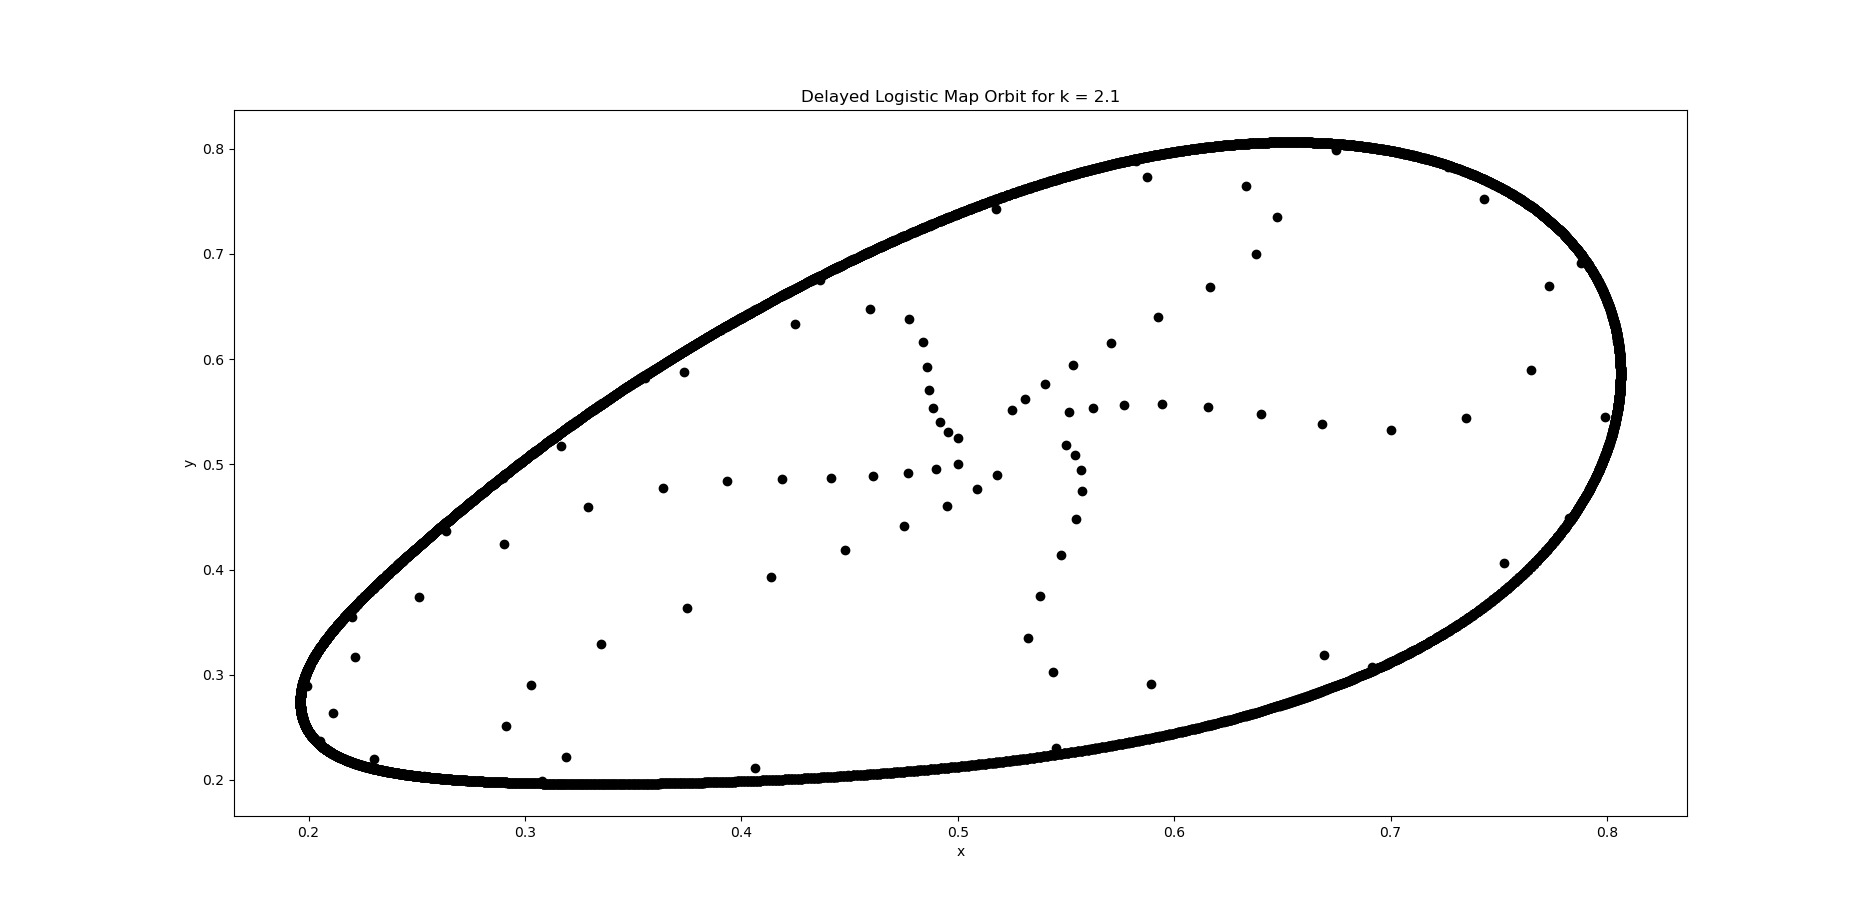
\includegraphics[scale=0.35]{variation.png}
	\centering
	\caption{Delayed Logistic Map with $k=2.1$ and Seed $(0.5,0.5)$}\label{fig:5}
	\centering
\end{figure}

There are some initial conditions for which $y_n\to -\infty$, even though we have $k<k_{\infty}$. This implies that the basin for attraction does not extend very far, since not only must it be confined within $[0,1]\times [0,1]$, but generally seeds far above the attractor will diverge.

It can be reasonably assumed the same holds for all attractors of $F$, but with varying basins of attraction. Additionally, large seeds for  $k<2$ can also diverge, similarly to that of $k=2.1$.
\section{Discussion}\label{sec:4}
Recall that \eqref{eq:7} was originally introduced as a possible model for the evolution of some species. The biological impacts of our analysis are very interesting, should this system be applicable in the real world. To summarize, we have found the following to be true for a small seed:
\begin{itemize}
	\item For $1.5\leq k<2$, $y_n$ converges to $\frac{k-1}{k}$.
	\item For $2<k<k_\infty\approx 2.271$, the system is likely chaotic, but at least has a large and possibly infinite number of periodic values. The collection of all of these values appears to resemble a smooth simmple closed curve.
	\item For $k_\infty\leq k$, the system diverges to $y_n\to -\infty$.
\end{itemize}
If we think of $k$ as a growth rate, then this implies for small enough values of $k$, a species growing subject to \eqref{eq:7} would eventually reach a stable population size. For a larger growth rate, the population may oscillate chaotically, never reaching a single fixed size. If $k$ grows too large, it could be that the population briefly exceeds the carrying capacity of the system. This results in the system plummeting to a negative value, which would equate biologically to a mass-extinction event.

We also found that for seeds far from the attractor or fixed point to diverge, meaning that very unstable initial populations may never reach stability, or even chaotic meta-stability, and may instead instantly die out.

I'm fairly unhappy that I did not have time to complete everything I wanted to complete. I had a previous version of the writeup that was much more straightforward and much less handwavy, but unfortunately I mistakenly thought the attractor would be a 1 dimensional object in $\mathbb{R}$, and only realized my mistake after completing a much more indepth numerical investigation of property 3 in definition \ref{dfn:1} than I was able to replicate after the fact. Originally, I had formally defined $\mu_\ell $ as a measure on some subset of $[0,1]$, and showed that $(A,\Sigma ,\mu_\ell )$ formed a measure space for $\Sigma $ the set of Lebesgue-measurable subsets of $A$ and finite $p$. Although this is a very minor detail as you don't need a formal measure function, it was still an interesting method that I wanted to include more formally than I was able to.

I also did not have time to complete the numerics as I would have liked, and due to the intense computational costs, I don't believe I would have been able to compute meaningfully small values to be able to say substantial things about the assignment. However, it was very interesting to have to think about how to numerically approach problems in the very non-numerical subject of topology, and although I wish I had more time to clean up the explanation of my methods, I still think it was very cool. It was also very interesting how little literature existed on the delayed logistic difference equation, and most of the few articles I could find were far above my level and were largely considering more complex variants of equation \eqref{eq:7}.
\appendix
\section{Code}
\begin{center}
	Code 1: Binary Search Algorithm for Infinity Bifurcation\label{code:1}
\end{center}
\begin{lstlisting}[language=Python]
interval = (2.1,2.5) # interval inside which the bifurcation occurs
x_init = 0.1 # initial x value
y_init = 0.2 # initial y value
iterations = 200 # number of iterations to guarentee precision to
fig, ax = plt.subplots()
precision = 1e-20 # precision of decimal

# returns True if y goes negative for this k value, fales otherwise
def negative(k, it):
    x_vals = [x_init]
    y_vals = [y_init]
    for _ in range(it):
        x, y = DDE(x_vals[-1], y_vals[-1], k)
        x_vals.append(x)
        y_vals.append(y)
        if y < 0:
            return True
    return False

# performs a binary search for bifurcation point
def find_infinity(start, end, precision, it):
    while end - start > precision:
        mid = (start + end) / 2
        if negative(mid, iterations):
            end = mid
        else:
            start = mid
        return (start + end) / 2

def main():
    bifurcation_point = find_infinity(interval[0], interval[1], precision, iterations)
    print(f"Bifurcation point: k = {bifurcation_point}")

if __name__ == "__main__":
    main()
\end{lstlisting}
\begin{center}
	Code 2: Bifurcation Diagram for Delayed Logistic Map\label{code:2}
\end{center}
\begin{lstlisting}[language=Python]
#!/usr/bin/env python3

import numpy as np
import matplotlib.pyplot as plt

interval = (1.5, 2.27)  # start, end
accuracy = 0.00002
reps = 100000  # number of repetitions
numtoplot = 100
lims = np.zeros(reps)

fig, ax = plt.subplots()
fig.set_size_inches(16, 9)

lims[0] = 0.1
lims[1] = 0.2
for r in np.arange(interval[0], interval[1], accuracy):
    for i in range(reps - 1):
        lims[i + 1] = r * lims[i] * (1 - lims[i-1])

    ax.plot([r] * numtoplot, lims[reps - numtoplot:], ".", color="black", markersize=0.1)


ax.set(xlabel="k", ylabel="y", title="Delayed Logistic Map Bifurcation Diagram")
plt.show()
\end{lstlisting}
This code is inspired by Wikipedia code for visualizing the regular logistic map \cite{wiki}. The code has been modified to implement the delayed variant of the logistic map, and to increase accuracy. Specifically, I increased the number of iterations of $k$ along the interval $[1.5,2.27]$ by 5x, and increased the number of repetitions of the delayed logistic map by over 100x of the original.

Since I basically stole the code, I will explain how it works to show I understand what is happening. The code works by iterating the delayed logistic map 100000 times and plotting the last 100 values. If the map is approaching a stable solution, we should see the points clustering around that solution, which will shade the graph a darker color. If the points are not approaching a solution, we should see a distribution of lighter colored points.
\begin{center}
	Code 3a: Identifying Arclength of $A$\label{code:3a}
\end{center}
\begin{lstlisting}[language=Python]
def main4():
    x_vals = [x_init]
    y_vals = [y_init]
    for _ in range(iterations):
        x, y = DDE(x_vals[-1], y_vals[-1], 2.1)
        x_vals.append(x)
        y_vals.append(y)

    x_vals = x_vals[100:]
    y_vals = y_vals[100:]

    points = np.array(list(zip(x_vals, y_vals)))
    num_points = len(points)
    ordered_points = [points[0]]
    visited = np.zeros(num_points, dtype=bool)
    visited[0] = True

    for _ in range(1, num_points):
        last_point = ordered_points[-1]
        distances = np.linalg.norm(points - last_point, axis=1)
        distances[visited] = np.inf

        nearest_idx = np.argmin(distances)
        ordered_points.append(points[nearest_idx])
        visited[nearest_idx] = True

    ordered_points = np.array(ordered_points)

    arclength = np.sum(np.linalg.norm(np.diff(ordered_points, axis=0), axis=1))
    print(f"Arclength: {arclength}")
\end{lstlisting}
\begin{center}
	Code 3b: Approximating Density in $A$\label{code:3b}
\end{center}
\begin{lstlisting}
def main4(its):
    x_vals = [x_init]
    y_vals = [y_init]
    for _ in range(its):
        x, y = DDE(x_vals[-1], y_vals[-1], 2.1)
        x_vals.append(x)
        y_vals.append(y)

    x_vals = x_vals[100:]
    y_vals = y_vals[100:]

    points = np.array(list(zip(x_vals, y_vals)))
    num_points = len(points)
    ordered_points = [points[0]]
    visited = np.zeros(num_points, dtype=bool)
    visited[0] = True

    diameter = 2 * arclength / (its - 100)

    for _ in range(1, num_points):
        last_point = ordered_points[-1]
        distances = np.linalg.norm(points - last_point, axis=1)
        distances[visited] = np.inf

        nearest_idx = np.argmin(distances)
        ordered_points.append(points[nearest_idx])
        visited[nearest_idx] = True

    ordered_points = np.array(ordered_points)
    l_measure = 0

    for i in range(len(ordered_points) - 1):
        p1 = ordered_points[i]
        p2 = ordered_points[i + 1]
        dist = np.linalg.norm(p2 - p1)
        if dist > diameter:
            l_measure += dist

    #print(f"L-measure is {l_measure / arclength}")
    return l_measure


measures = []
things = np.arange(interval_2[0], interval_2[1], accuracy_2)
for its in things:
        measures.append(main4(its) / arclength)
        print(f"Completed for {its}")
plt.plot(things, measures)
plt.show()
\end{lstlisting}
\bibliographystyle{plain}
\bibliography{refs2.bib}
\end{document}
